
\section{Testowanie automatyczne} \ \ \

Proces testowania jest bardzo istotny przy weryfikacji, czy oprogramowanie będzie działać zgodnie z oczekiwaniami klienta. W związku z tym testowanie powinno być skuteczne w znajdowaniu błędów oraz przebiegać z użyciem jak najmniejszych kosztów (czasowych i pieniężnych). Trzeba pamiętać jednak, że nawet jeżeli oprogramowanie zostanie przetestowane, to i tak mogą występować w nim błędy. Im później wykryje się nieprawidłowe działania programu, tym więcej będzie kosztować jego naprawienie. Jeżeli w oprogramowaniu występuje dużo błędów, oznacza to, że nie zostało ono dokładnie przetestowane. 

\begin{figure}[H]
\centering
\captionsetup{justification=centering}
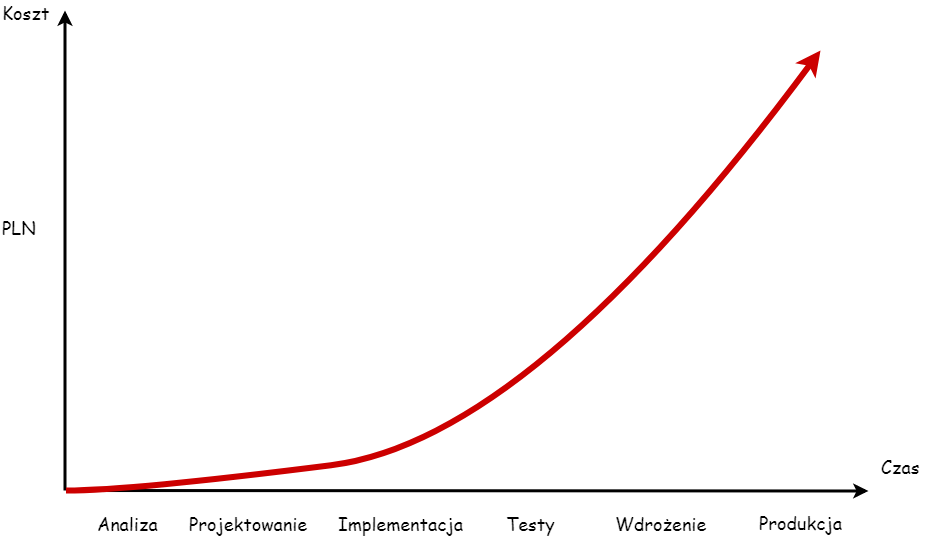
\includegraphics[width=1\textwidth]{Diagram.png}
\caption[Wykres zależności między czasem wykrycia błędu w projekcie a kosztem związanym z jego naprawieniem]{\label{fig:ham}Wykres zależności między czasem wykrycia błędu w projekcie a kosztem związanym z jego naprawieniem \\ źródło: opracowanie własne na podstawie \cite{smiglin}}
\end{figure}

 Jest wiele możliwości, żeby zapobiec takiej sytuacji. Jedną z nich, na której skupimy się w tym rozdziale, jest \textbf{automatyzacja testowania}, inaczej użycie oprogramowania do wykonania bądź wspierania czynności testowych w celu kontrolowania wykonania testu, porównania rezultatów rzeczywistych z oczekiwanymi, ustawienia warunków wstępnych testu i innych funkcji kontroli i raportowania testów. \cite{roman}


\subsection{Zalety automatyzacji}

Istnieje mnóstwo korzyści płynących z automatyzacji testowania, wśród których można wymienić (\cite{io}):

\begin{itemize}
\item zmniejszenie kosztów testowania względem manualnego wykonywania przypadków testowych, ponieważ powtarzalne i monotonne zadania mogą zostać zastąpione przez skrypty automatyzujące;
\item wykonanie testów regresyjnych dla nowej wersji oprogramowania (pod warunkiem, że tego typu zestaw testowy został już przygotowany i zautomatyzowany dla wcześniejszej wersji) - łatwiej i szybciej można wykryć potencjalne problemy powstałe w wyniku dokonanych zmian;
\item szybkość działania - jako że testy automatyczne wykonują się szybko, można je uruchamiać częściej i o każdej porze dnia (na przykład w nocy lub też w dzień wolny od pracy);
\item parametryzację, dzięki której można przez poszerzyć zestaw testów, a co za tym idzie dokładniej sprawdzić oprogramowanie;
\item skupienie się na projektowaniu innych, lepszych testów;
\item przewidywalność testów - skrypty testowe zawierają kroki, które wykonają się za każdym razem w dokładnie ten sam sposób;
\item możliwość testowania na różnym sprzęcie, w różnych konfiguracjach, na różnych bazach danych;
\item umożliwienie wykonania pewnych rodzajów testów, które są bardzo trudne bądź niemożliwe do przetestowania manualnie, np. testy wydajności czy obciążeniowe.
\end{itemize}


\subsection{Wady automatyzacji} 

Tak jak wszystko, automatyzacja testowania ma również słabe strony, takie jak:
\begin{itemize}
\item duży koszt wytworzenia testów (2-10 razy większy niż przy testach manualnych);
\item przy częstych zmianach w oprogramowaniu należy testy dostosować do kolejnej wersji, co oznacza poświęcenie nieraz dodatkowego czasu oraz pieniędzy na ich modyfikację;
\item znajdują mało błędów w stosunku do testów manualnych - wynika to z faktu, że automatyzujemy tylko wtedy, gdy rozważany scenariusz wykonany ręcznie działa prawidłowo;
\item nie wszystkie testy da się zautomatyzować, np. testy użyteczności czy interfejsu graficznego;
\item nie opłaca się automatyzować wszystkich przypadków, zwłaszcza tych, które są wykonywane rzadko.
\end{itemize}


\subsection{Matematyczny punkt widzenia}

Na testy automatyczne możemy spojrzeć jako na automaty skończone, za pomocą których można opisać nie tylko same testy, ale także całą architekturę automatyzacji. W tym podrozdziale podana zostanie definicja wraz z przykładem.

\begin{df}
\textbf{Automat skończony} (ang. \textit{finite state machine}, \textit{FSM}) jest matematycznym modelem obliczeniowym, który składa się ze skończonej liczby stanów oraz przejść pomiędzy nimi, a także z towarzyszącymi im akcjami. \cite{auto}. Przejścia między kolejnymi stanami automatu można opisać za pomocą \textbf{diagramu stanów}.

\newpage

\noindent Automaty skończone można podzielić na:
\begin{itemize}
    \item \textbf{deterministyczne} (ang. \textit{deterministic finite automation}, \textit{DFA}) - dla aktualnego stanu wiemy, jaki będzie kolejny i że wystąpi dokładnie jeden; brak losowości w wyborze.
    \item \textbf{niedeterministyczne} (ang. \textit{non-deterministic finite automation}, \textit{NFA}) - dla aktualnego stanu możliwe jest, że będzie więcej niż jeden następny stan, który ponadto może zostać wybrany losowo i równolegle.
\end{itemize}


\noindent Formalnie automat skończony możemy opisać jako piątkę $(S,\Sigma, s_0, \delta, F)$, gdzie:
\begin{itemize}
    \item $S$ - niepusty i skończony zbiór stanów.
    \item $\Sigma$ - skończony alfabet wejściowy.
    \item $s_0$ - stan początkowy, przy czym $s_0 \in S$.
    \item $\delta$ - funkcja przejścia opisana jako $\delta: S \times \Sigma \rightarrow S$ (dla niedeterministycznych automatów skończonych $\delta: S \times \Sigma \rightarrow P(S)$, gdzie $P(S)$ jest zbiorem potęgowym zbioru $S$).
    \item $F$ - zbiór stanów akceptowalnych (końcowych), przy czym $F \subseteq S$.
\end{itemize}

\begin{prz}
Rozważmy następujący automat skończony, który opisuje schemat działania skryptu testowego:


\begin{figure}[H]
\centering
\captionsetup{justification=centering}
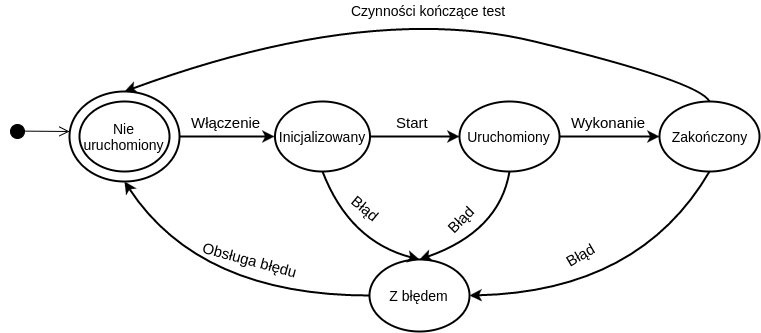
\includegraphics[width=1\textwidth]{AutoTestFSM.png}
\caption[Automat skończony dla tes/'tu automatycznego]{\label{fig:autfsm}Automat skończony dla testu automatycznego \\ źródło: opracowanie własne}
\end{figure}


Stan \textit{Nieuruchomiony} jest stanem startowym i zarazem końcowym. Test jest \textit{Inicjalizowany}, gdy go uruchomimy, czyli wtedy jest przygotowywane środowisko, wczytywane dane testowe oraz wykonywane są inne operacje przed wykonaniem testu. Następnie test jest w stanie \textit{Uruchomiony}, czyli wykonuje kolejno kroki testowe. Przechodzi wtedy do stanu \textit{Zakończony}, a następnie są robione czynności kończące test, takie jak czyszczenie danych czy usuwanie rekordów z tabeli, które istniały tylko na potrzeby testowania. Na sam koniec test automatyczny wraca do stanu początkowego, czyli znowu jest \textit{Nieuruchomiony}.


W przypadku, gdy wystąpi błąd przy inicjalizacji, uruchomieniu czy zakończeniu testu, wtedy ma stan \textit{Z błędem}. W ramach tego znaleziony defekt zostaje poddany obsłudze, a następnie przechodzi do stanu początkowego - \textit{Nie uruchomiony}.


Jeżeli powyższy automat rozważamy jako piątkę $(S,\Sigma, s_0, \delta, F)$, to wtedy:
\begin{itemize}
    \item $Q$ = $\{$Nieuruchomiony, Inicjalizowany, Uruchomiony, Zakończony, Z błędem$\}$
    \item $\Sigma$ = $\{$Włączenie, Start, Wykonanie, Czynności kończące test, Błąd, Obsługa błędu$\}$ 
    \item $q_0$ = Nieuruchomiony
    \item $F$ = $\{$Nieuruchomiony$\}$
    \item $\delta$ - funkcję przejścia opiszemy za pomocą diagramu stanów
\end{itemize}

\begin{table}[H]
\centering
\caption{Diagram stanów dla powyższego deterministycznego automatu skończonego}
\label{my-label}
\resizebox{\textwidth}{!}{%
\begin{tabular}{|l|l|l|l|l|l|l|}
\hline
\rowcolor[HTML]{9B9B9B} 
                                       & Włączenie      & Start       & Wykonanie  & Czynności kończące test & Błąd     & Obsługa błędu  \\ \hline
\cellcolor[HTML]{9B9B9B}Nieuruchomiony & Inicjalizowany &             &            &                         &          &                \\ \hline
\cellcolor[HTML]{9B9B9B}Inicjalizowany &                & Uruchomiony &            &                         & Z błędem &                \\ \hline
\cellcolor[HTML]{9B9B9B}Uruchomiony    &                &             & Zakończony &                         & Z błędem &                \\ \hline
\cellcolor[HTML]{9B9B9B}Zakończony     &                &             &            & Nieuruchomiony          & Z błędem &                \\ \hline
\cellcolor[HTML]{9B9B9B}Z błędem       &                &             &            &                         &          & Nieuruchomiony \\ \hline
\end{tabular}%
}
\end{table}


\end{prz}

\end{df}



\subsection{Podsumowanie}

Przedstawiono zarówno zalety, jak i wady procesu automatyzacji testowania. Dzięki temu można wysunąć następujące wnioski:
\begin{itemize}
    \item Pewne rodzaje testów należy automatyzować, takie jak testy wydajności, testy API czy testy jednostkowe.
    \item Automatyzację należy traktować jako uzupełnienie testów manualnych - najpierw należy wykonać przypadek ręcznie, a dopiero potem pisać program, który wykona działający już scenariusz testowy.
    \item Scenariusze testowe zautomatyzowane szybciej się wykonają niż gdyby je wykonać manualnie.
    \item Zmniejszenie kosztów nawet do $80\%$ związanego z manualnym przetestowaniu oprogramowania pozwala na dokładniejsze jego sprawdzenie poprzez dodanie większej ilości przypadków testowych oraz możliwość dobrania więcej danych testowych.
    \item Warto automatyzować takie czynności testowe, jak porównywanie wyników oczekiwanych z rzeczywistymi czy wykonywanie powtarzalnych kroków testowych.
\end{itemize}